\chapter{Evaluation}\label{ch:evaluation}
In this chapter, the individual algorithms, as well as the final performance of the combined system, will be evaluated.
The depth from motion algorithm will be evaluated based on different materials and their resulting confidence maps in section~\ref{sec:eval-depth-from-motion}.
In section~\ref{sec:eval-ransac-algorithm}, the RANSAC algorithm will be evaluated based on synthetic data, as well as real world data.
Finally, in section~\ref{sec:eval-combined}, the combined system performance will be evaluated.
%klare begründung => Anforderung erfüllt ja oder nein

\section{Depth from Motion}\label{sec:eval-depth-from-motion}
As the depth from motion algorithm greatly differs in its performance based on the amount of texture in the captured scene~\cite{google_llc_arcore_doc},
this section will evaluate different materials based on their resulting confidence maps, as retrieved from the ARCore Raw Depth API\@.
In figure~\ref{fig:materials}, the confidence maps of different materials are shown - the camera image on top, the confidence map on the bottom.

\begin{figure}[h!t]
    \centering
    % First row
    \begin{subfigure}[b]{0.25\textwidth}
        \centering
        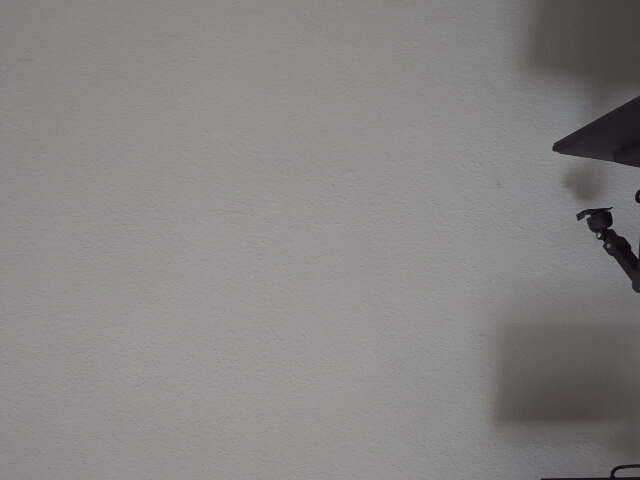
\includegraphics[width=0.9\linewidth]{images/materials/wall-far-cam}
    \end{subfigure}%
    \begin{subfigure}[b]{0.25\textwidth}
        \centering
        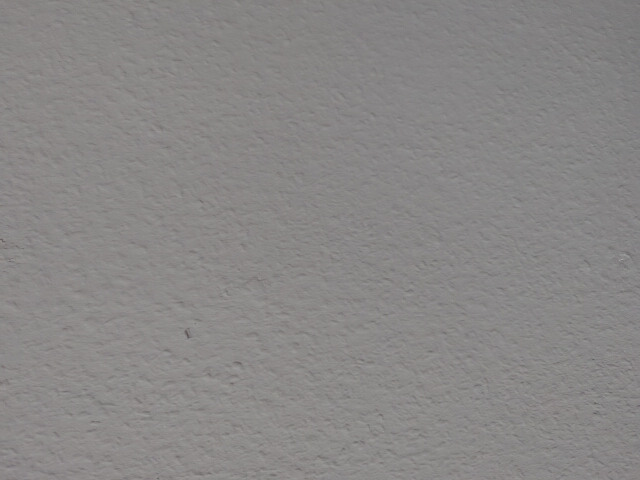
\includegraphics[width=0.9\linewidth]{images/materials/wall-close-cam}
    \end{subfigure}%
    \begin{subfigure}[b]{0.25\textwidth}
        \centering
        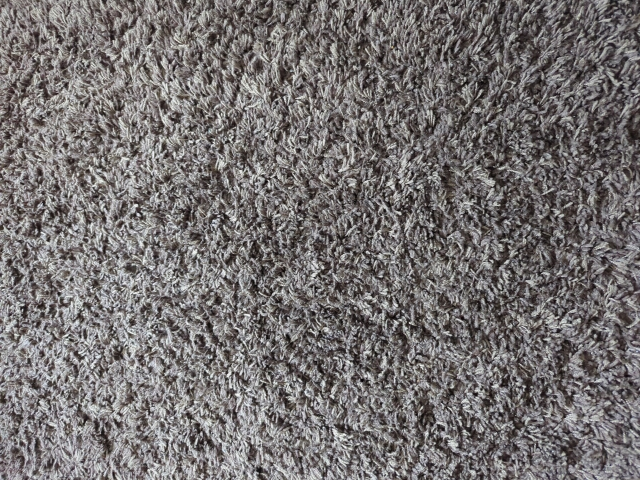
\includegraphics[width=0.9\linewidth]{images/materials/carpet-cam}
    \end{subfigure}%
    \begin{subfigure}[b]{0.25\textwidth}
        \centering
        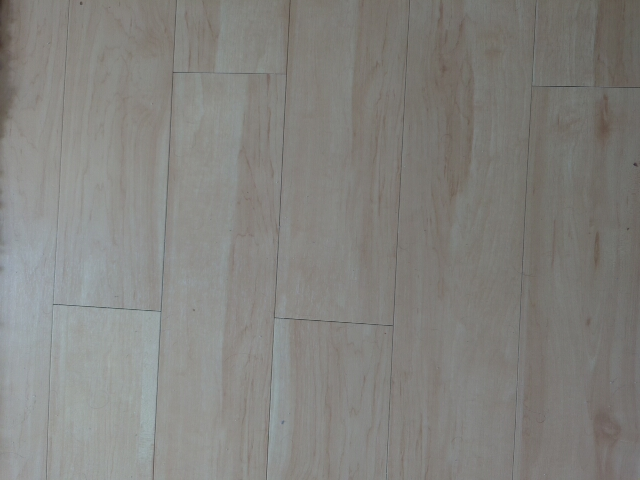
\includegraphics[width=0.9\linewidth]{images/materials/wood-cam}
    \end{subfigure}%

    \begin{subfigure}[b]{0.25\textwidth}
        \centering
        
\includegraphics[width=0.9\linewidth]{images/materials/wall-far-conf}
        \caption{Wall, 1.5m}
        \label{fig:material-wall-far}
    \end{subfigure}%
    \begin{subfigure}[b]{0.25\textwidth}
        \centering
        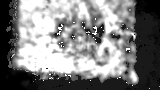
\includegraphics[width=0.9\linewidth]{images/materials/wall-close-conf}
        \caption{Wall, 0.5m}
        \label{fig:material-wall-close}
    \end{subfigure}%
    \begin{subfigure}[b]{0.25\textwidth}
        \centering
        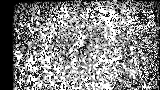
\includegraphics[width=0.9\linewidth]{images/materials/carpet-conf}
        \caption{Carpet}
        \label{fig:material-carpet}
    \end{subfigure}%
    \begin{subfigure}[b]{0.25\textwidth}
        \centering
        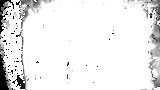
\includegraphics[width=0.9\linewidth]{images/materials/wood-conf}
        \caption{Wooden floor}
        \label{fig:material-wood}
    \end{subfigure}%

    \vspace{0.5em}

    % First row
    \begin{subfigure}[b]{0.25\textwidth}
        \centering
        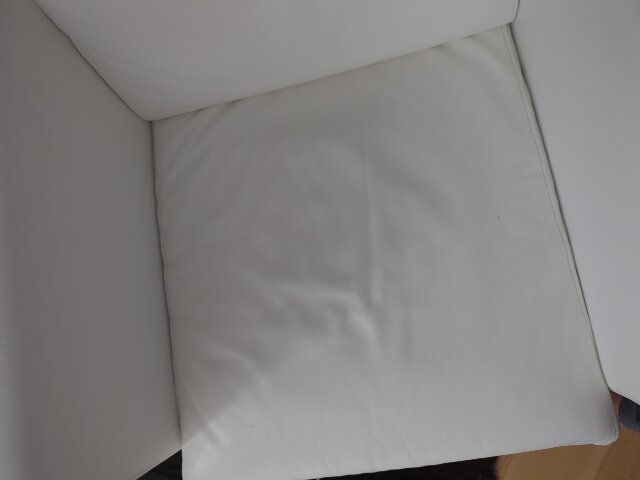
\includegraphics[width=0.9\linewidth]{images/materials/leather-cam}
    \end{subfigure}%
    \begin{subfigure}[b]{0.25\textwidth}
        \centering
        
\includegraphics[width=0.9\linewidth]{images/materials/whiteFurniture-cam}
    \end{subfigure}%
    \begin{subfigure}[b]{0.25\textwidth}
        \centering
        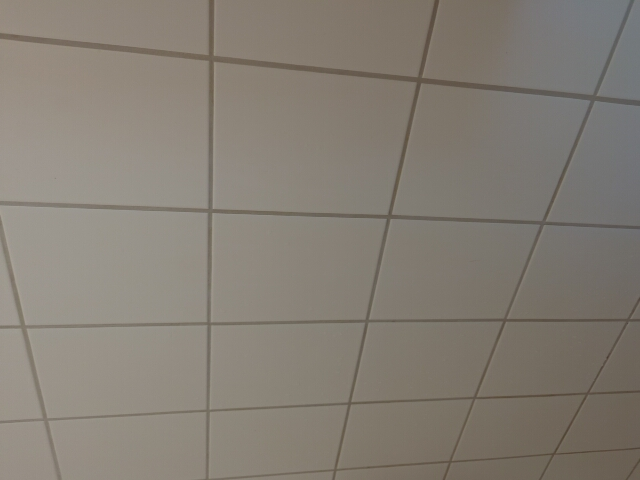
\includegraphics[width=0.9\linewidth]{images/materials/tiles-cam}
    \end{subfigure}%
    \begin{subfigure}[b]{0.25\textwidth}
        \centering
        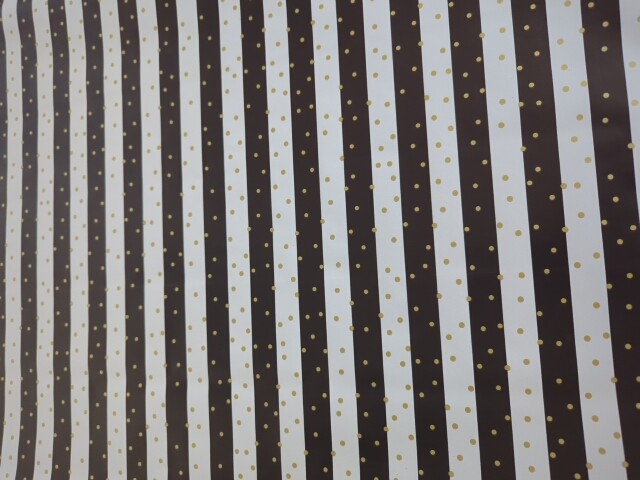
\includegraphics[width=0.9\linewidth]{images/materials/giftpaper-cam}
    \end{subfigure}%

    \begin{subfigure}[b]{0.25\textwidth}
        \centering
        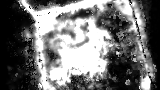
\includegraphics[width=0.9\linewidth]{images/materials/leather-conf}
        \caption{Leather armchair}
        \label{fig:material-leather}
    \end{subfigure}%
    \begin{subfigure}[b]{0.25\textwidth}
        \centering
        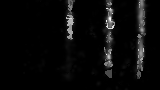
\includegraphics[width=0.9\linewidth]{images/materials/whiteFurniture-conf}
        \caption{White furniture}
        \label{fig:material-whiteFurniture}
    \end{subfigure}%
    \begin{subfigure}[b]{0.25\textwidth}
        \centering
        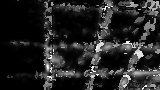
\includegraphics[width=0.9\linewidth]{images/materials/tiles-conf}
        \caption{Bathroom tiles}
        \label{fig:material-tiles}
    \end{subfigure}%
    \begin{subfigure}[b]{0.25\textwidth}
        \centering
        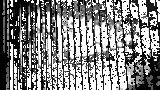
\includegraphics[width=0.9\linewidth]{images/materials/giftpaper-conf}
        \caption{Gift paper}
        \label{fig:material-giftpaper}
    \end{subfigure}%

    \caption{Comparison of confidence maps of different materials. Camera image on top, confidence map on bottom.}
    \label{fig:materials}
\end{figure}

In figure~\ref{fig:material-wall-close} and~\ref{fig:material-wall-far}, the confidence maps of a wall at different distances are shown.
It is apparent that the confidence of the wall at 1.5m distance is almost completely black, meaning low confidence.
This is due to the lack of any texture on the wall at this distance.
When moving closer to the wall, the structure of the wall becomes more apparent and the confidence increases greatly.

In figure~\ref{fig:material-carpet}, a carpet with a lot of texture is shown, the resulting confidence map has fairly high confidence on average,
but also has dark sports throughout the map.
This could be a result of the repetitive pattern of the carpet.

The highest confidence of all tested materials is achieved on a wooden floor, as shown in figure~\ref{fig:material-wood}.
This can be attributed to the high amount of texture and value variance through the wood, while not being repetitive.
The seams between the wooden planks are also clearly visible.

Figure~\ref{fig:material-leather} shows a leather armchair, which has a high confidence on the seams of the chair and
on creases of the leather, with low confidence in other areas, where the leather is smoother.
A similar pattern is visible on white furniture and bathroom tiles, in figures~\ref{fig:material-whiteFurniture} and~\ref{fig:material-tiles} respectively,
where the white surface has very low confidence, while the seams between the surfaces have increased confidence.
The gift paper shown in figure~\ref{fig:material-giftpaper} shows a similar effect, but less pronounced.
As the surface itself is striped with dots randomly placed throughout, the confidence is higher overall,
but the striped pattern is still visible in the confidence map, as the stripes themselves contain little texture.

These examples show how the amount of texture on a given surface greatly influences the confidence of the depth from motion algorithm, as expected.
The algorithm performs best on surfaces with high texture, while struggling with low texture surfaces.
Small repetitive patterns can also lead to low confidence, as visible in the carpet example.
It is also important to note that the texture captured by the camera itself is important, not the texture of the material itself.
This can be seen in the first example of the wall: When capturing from afar, the cameras resolution is too low to capture the texture,
but when moving closer to the wall, the texture of the wall becomes more apparent and the confidence increases.
Lighting conditions will also influence the confidence of the algorithm,
as angled light will create shadows that will increase the texture of the surface~\cite{google_llc_arcore_doc} (not shown in the comparison).


\section{RANSAC Algorithm}\label{sec:eval-ransac-algorithm}
In this section, the RANSAC algorithm will be evaluated based on a model of a cube,
first using synthetic data in section~\ref{subsec:tests-on-singular-synthetic-cube} and then using real world data
in section~\ref{subsec:tests-on-real-world-data}.

\subsection{Tests on singular synthetic cube}\label{subsec:tests-on-singular-synthetic-cube}

A unit cube will be used as a test object to evaluate the RANSAC algorithm.
The cube has been generated with a side length of 1 and a sampling rate of 0.01.
This would equate to a cube with a side length of 1m and a distance of 1cm between points in the real world,
which is comparable to what is provided by the Raw Depth API\@.

\subsubsection{Resilience to Noise}
In figure~\ref{fig:test-noise}, the unit cube is shown with varying noise levels using gaussian noise.
The noise level is defined as the standard deviation of the noise added to the points.

With a noise level of 0.01, the cube is perfectly reconstructed.
Increasing the noise level to 0.02, the cube is still recognized mostly correctly.
Starting from noise level to 0.03, the default parameters do not yield correct results.
To achieve correct results, the epsilon parameter of the RANSAC algorithm has to be increased to 0.2.
This leads to 6 faces being recognized correctly, but some points not being assigned to the correct faces,
as the with each primitive extraction pass, points are extracted that lie within 0.2 of the recognized plane.


\begin{figure}[h!tp]
    \centering
    % First row
    \begin{subfigure}[b]{0.25\textwidth}
        \centering
        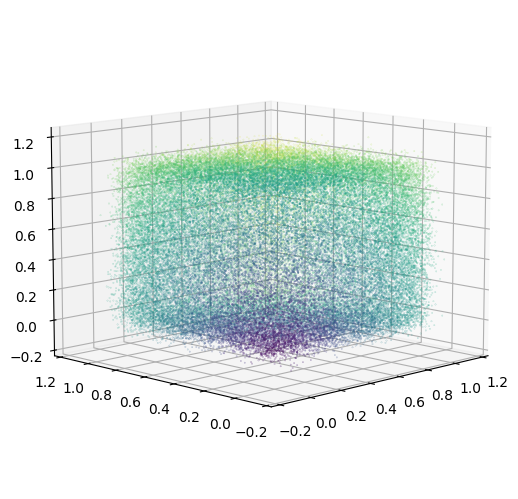
\includegraphics[width=0.9\linewidth]{python/plots/cube_points/data/cube_points}
    \end{subfigure}%
    \begin{subfigure}[b]{0.25\textwidth}
        \centering
        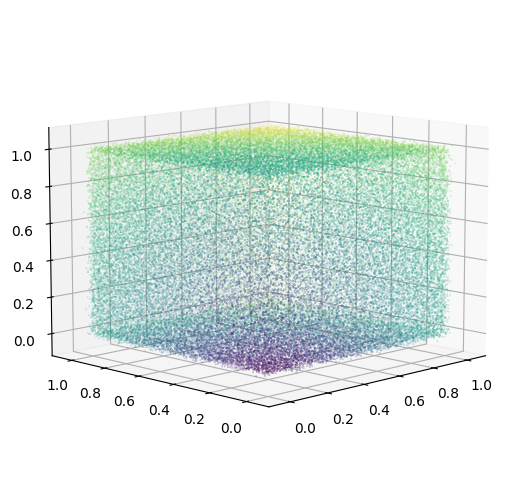
\includegraphics[width=0.9\linewidth]{python/plots/cube_points/data/noise/cube_points_noise_01}
    \end{subfigure}%
    \begin{subfigure}[b]{0.25\textwidth}
        \centering
        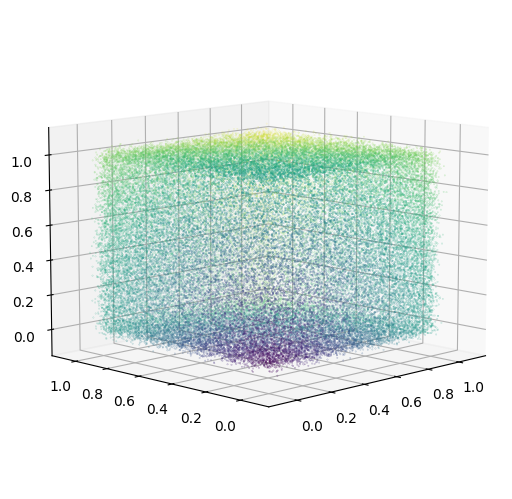
\includegraphics[width=0.9\linewidth]{python/plots/cube_points/data/noise/cube_points_noise_02}
    \end{subfigure}%
    \begin{subfigure}[b]{0.25\textwidth}
        \centering
        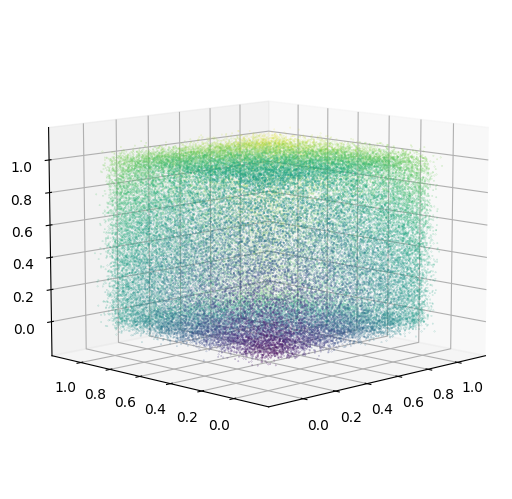
\includegraphics[width=0.9\linewidth]{python/plots/cube_points/data/noise/cube_points_noise_03}
    \end{subfigure}%

%    \vspace{0.5em}

    \begin{subfigure}[b]{0.25\textwidth}
        \centering
        
\includegraphics[width=0.9\linewidth]{python/plots/cube_points/data/cube_points_primitives}
        \caption{Noise level 0.00}
    \end{subfigure}%
    \begin{subfigure}[b]{0.25\textwidth}
        \centering
        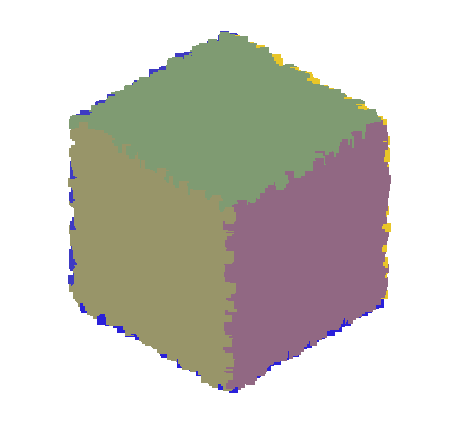
\includegraphics[width=0.9\linewidth]{python/plots/cube_points/data/noise/cube_points_noise_01_primitives}
        \caption{Noise level 0.01}
    \end{subfigure}%
    \begin{subfigure}[b]{0.25\textwidth}
        \centering
        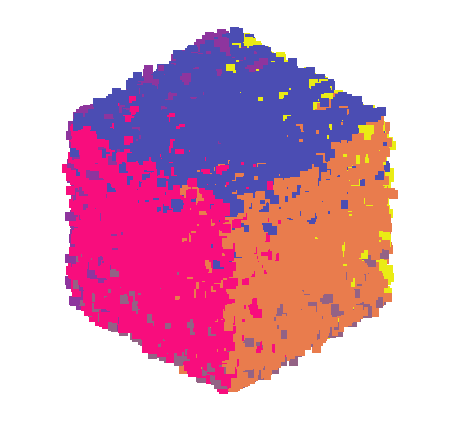
\includegraphics[width=0.9\linewidth]{python/plots/cube_points/data/noise/cube_points_noise_02_primitives}
        \caption{Noise level 0.02}
    \end{subfigure}%
    \begin{subfigure}[b]{0.25\textwidth}
        \centering
        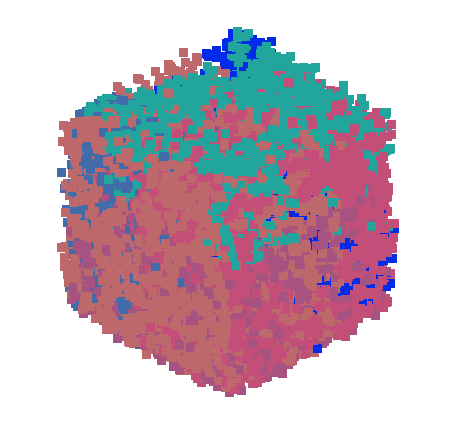
\includegraphics[width=0.9\linewidth]{python/plots/cube_points/data/noise/cube_points_noise_03_primitives}
        \caption{Noise level 0.03}
    \end{subfigure}%

    \caption{Unit cube with varying noise level}
    \label{fig:test-noise}
\end{figure}

\subsubsection{Resilience to Missing Data}

As a big problem of depth from motion techniques is the lack of depth information in areas with minimal texture,
the resilience to missing data is crucial.
In figure~\ref{fig:test-missing}, points towards the center of the cubes surfaces have been removed.
This mimics the structure of real world data from the Depth API,
as edges are often detected more accurately than surfaces.
%TODO: citation needed
To achieve this, points have been removed with an increasing probability based on the
quadratic distance to the center of the face the points belongs to.

The algorithm is able to correctly recognize the faces of the cube with a missing level up to 24.
With a missing level of 48, the algorithm still detects the planes, but doesn't assign all points to the faces.
With increasing missing level, the n parameter, which defines the minimum number of points required to fit a primitive,
is also required to be lowered.
In real world applications this would lead to more false detections, primitives being detected where there are none.

%Given a point $x$ with coordinates $(x_1, x_2, x_3)$, edge length $l$, and missing data rate $r$,
%the distance to the closest edge can be calculated as |
%
%As the cube is centered at the origin and aligned with the axis, the absolute of one coordinate will always equal $l/2$.
%By filtering out this coordinate, the point $x$ can be projected onto the plane of the cube,
%resulting in point $x'$ with coordinates $(x'_1, x'_2)$.
%
%The probability $p$ of a point being removed can then be calculated as

%\begin{equation}
%    p = \left(\frac{\sqrt{(l/2 - |x'_1|) \cdot (l/2 - |x'_2|)}}{l / 2}\right)^2 \cdot r
%\end{equation}

\subsubsection{Resilience to Noise and Missing Data}

When combining both noise and missing data, the quality of the detection is much worse.
In figure~\ref{fig:test-both}, the cube is shown with a noise level of 0.01 and varying missing levels.
With noise level 0.01 and missing level 6, the cube is still recognized correctly.
With missing level 12, more than 6 faces are being recognized, but all the points are still assigned to primitives.
This is explained by the fact that the parameterization of the planes is not accurate enough to fit all the points of the planes.
Thus, the algorithm only fits a subset of the points to the primitive and will create a new parameterization
for the remaining points.
To achieve results with these conditions, the epsilon parameter had to be increased to 0.015 to achieve any results at all.
Using a noise level of 0.02 with missing data yields no satisfactory results, even with tweaking the parameters.

\begin{figure}[h!tp]
    \centering
    % First row
    \begin{subfigure}[b]{0.25\textwidth}
        \centering
        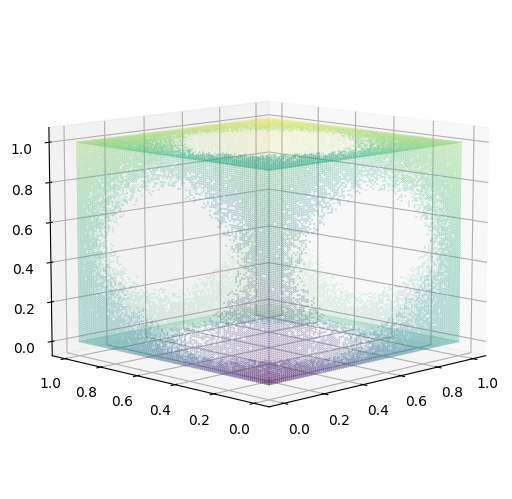
\includegraphics[width=0.9\linewidth]{python/plots/cube_points/data/missing/cube_points_missing_6_0}
    \end{subfigure}%
    \begin{subfigure}[b]{0.25\textwidth}
        \centering
        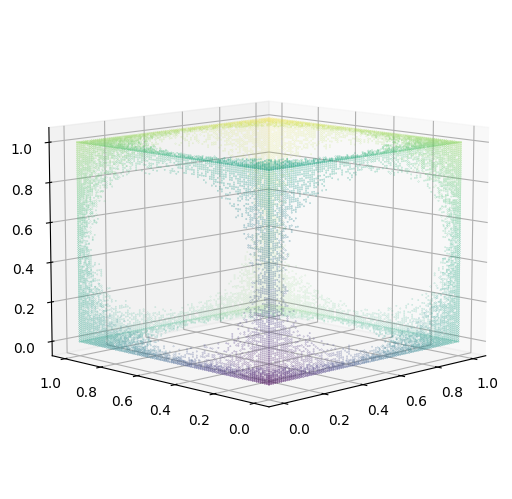
\includegraphics[width=0.9\linewidth]{python/plots/cube_points/data/missing/cube_points_missing_12}
    \end{subfigure}%
    \begin{subfigure}[b]{0.25\textwidth}
        \centering
        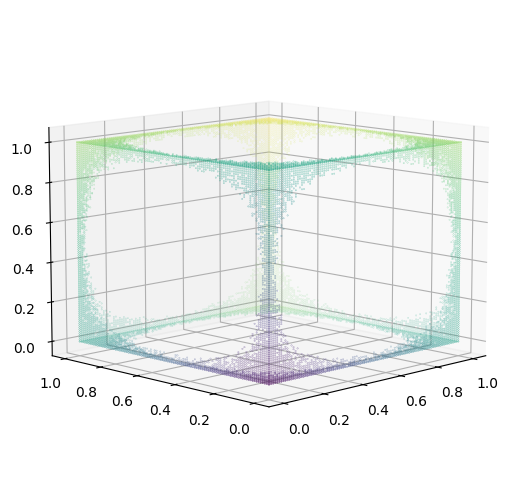
\includegraphics[width=0.9\linewidth]{python/plots/cube_points/data/missing/cube_points_missing_24}
    \end{subfigure}%
    \begin{subfigure}[b]{0.25\textwidth}
        \centering
        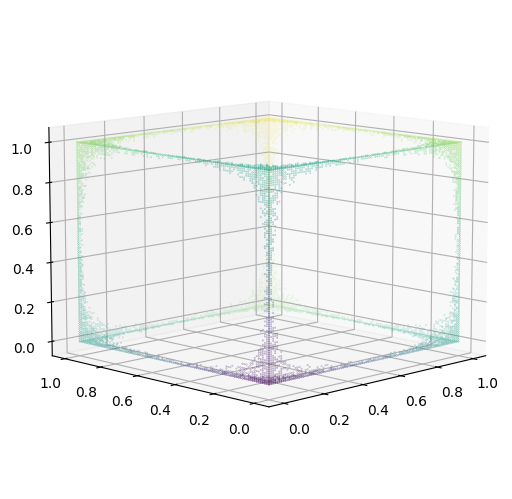
\includegraphics[width=0.9\linewidth]{python/plots/cube_points/data/missing/cube_points_missing_48}
    \end{subfigure}%

%    \vspace{0.5em}

    \begin{subfigure}[b]{0.25\textwidth}
        \centering
        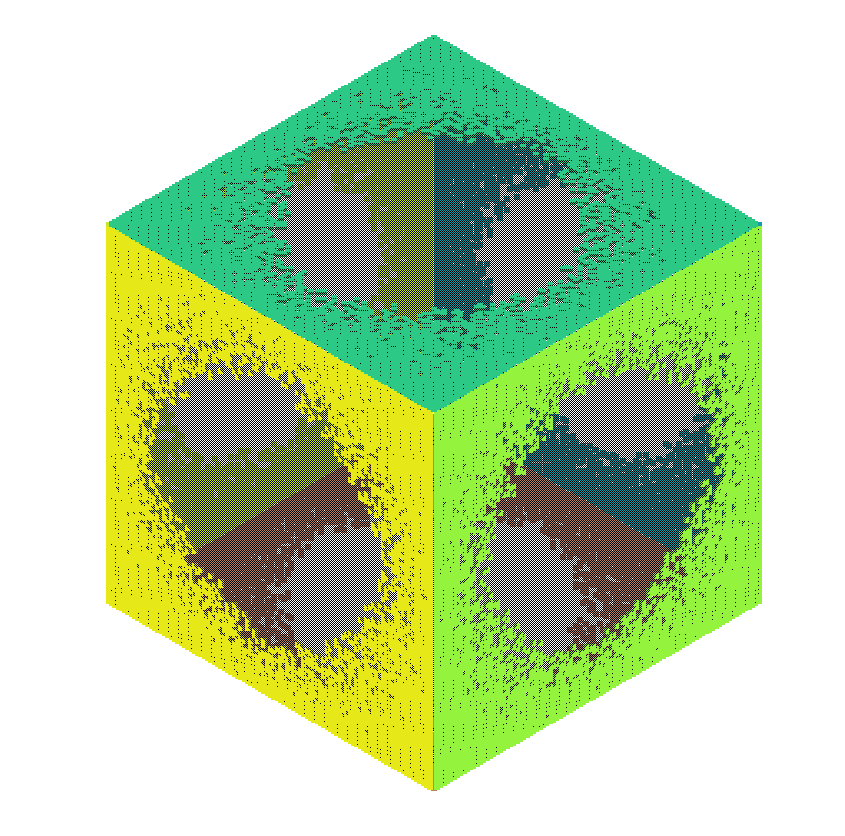
\includegraphics[width=0.9\linewidth]{python/plots/cube_points/data/missing/cube_points_missing_6_primitives}
        \caption{Missing level 6}
    \end{subfigure}%
    \begin{subfigure}[b]{0.25\textwidth}
        \centering
        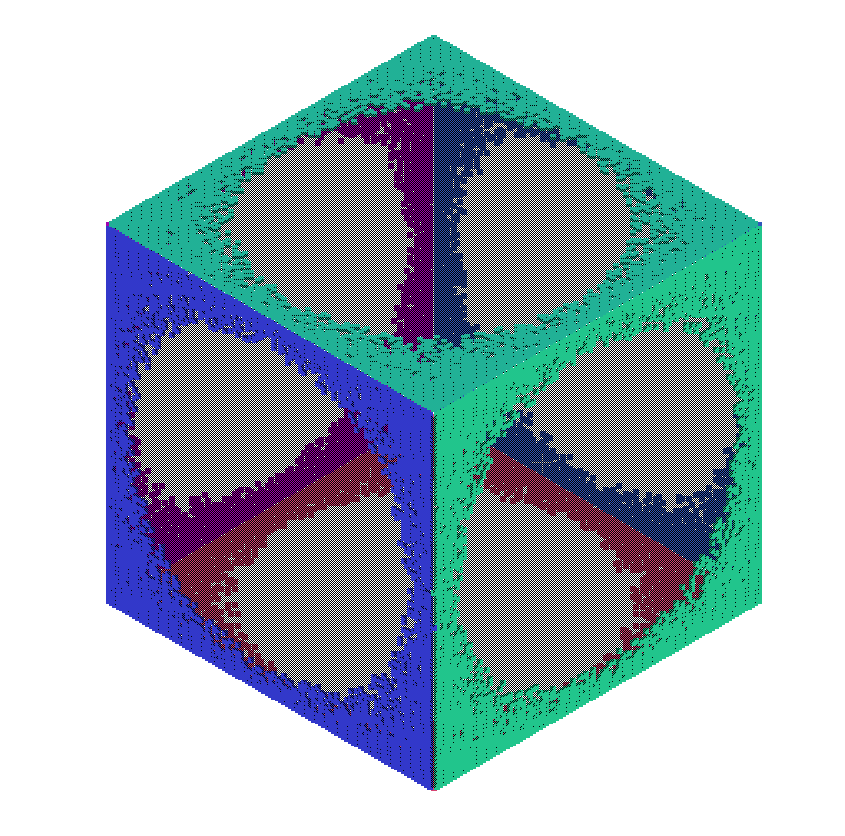
\includegraphics[width=0.9\linewidth]{python/plots/cube_points/data/missing/cube_points_missing_12_primitives}
        \caption{Missing level 12}
    \end{subfigure}%
    \begin{subfigure}[b]{0.25\textwidth}
        \centering
        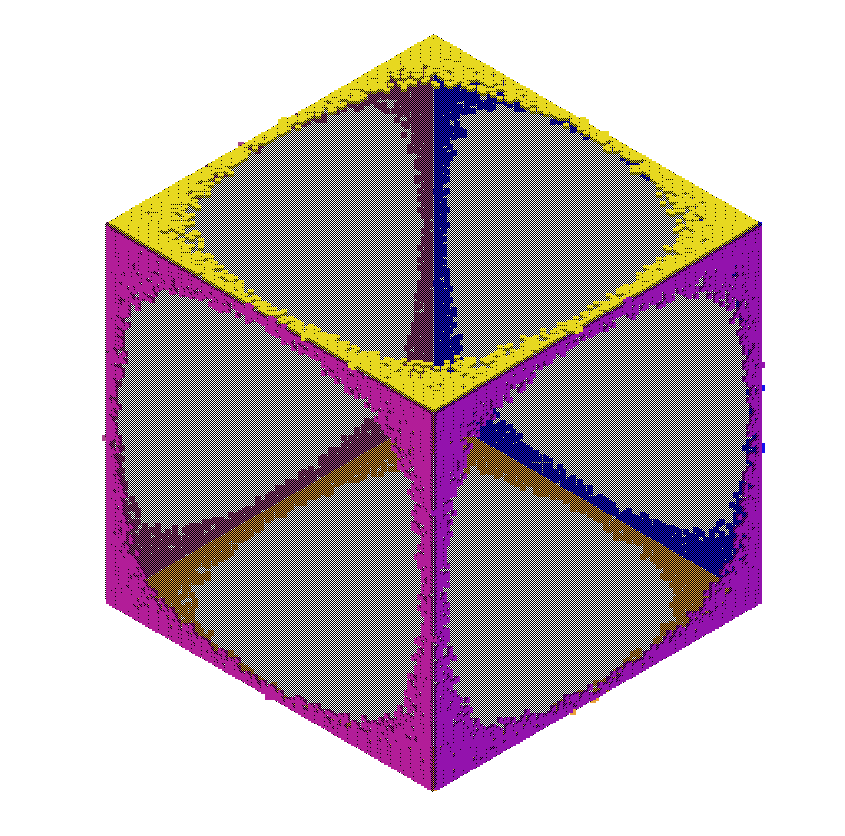
\includegraphics[width=0.9\linewidth]{python/plots/cube_points/data/missing/cube_points_missing_24_primitives}
        \caption{Missing level 24}
    \end{subfigure}%
    \begin{subfigure}[b]{0.25\textwidth}
        \centering
        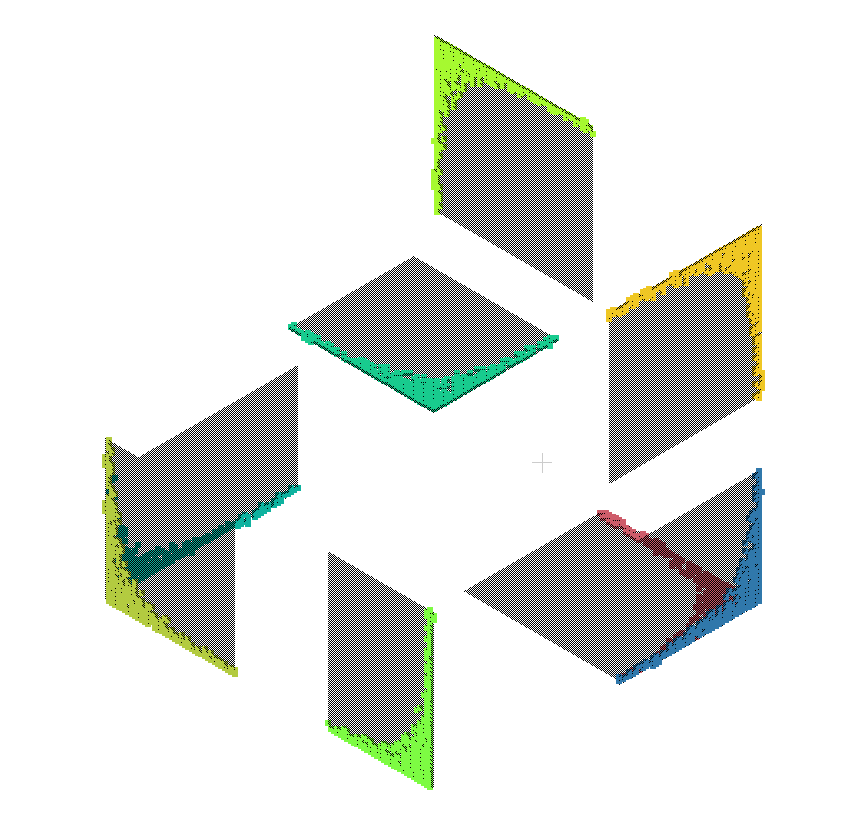
\includegraphics[width=0.9\linewidth]{python/plots/cube_points/data/missing/cube_points_missing_48_primitives}
        \caption{Missing level 48}
    \end{subfigure}%

    \caption{Unit cube with varying missing level}
    \label{fig:test-missing}
\end{figure}

\begin{figure}[ht!]

    \centering
    % First row
    \begin{subfigure}[b]{0.25\textwidth}
        \centering
        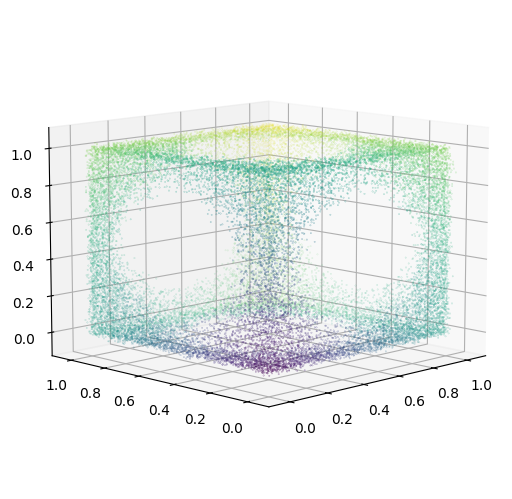
\includegraphics[width=0.9\linewidth]{python/plots/cube_points/data/matrix/cube_points_m6_n01}
    \end{subfigure}%
    \begin{subfigure}[b]{0.25\textwidth}
        \centering
        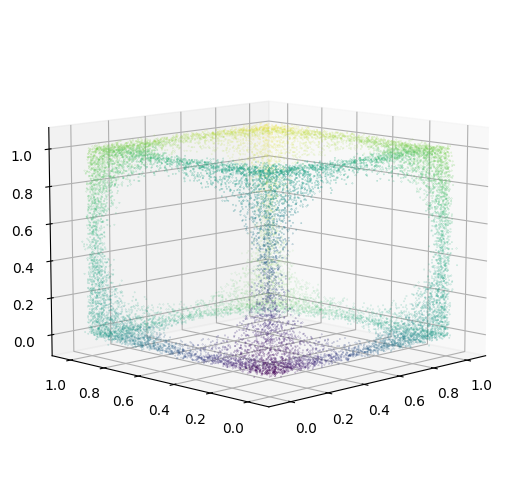
\includegraphics[width=0.9\linewidth]{python/plots/cube_points/data/matrix/cube_points_m12_n01}
    \end{subfigure}%
    \begin{subfigure}[b]{0.25\textwidth}
        \centering
        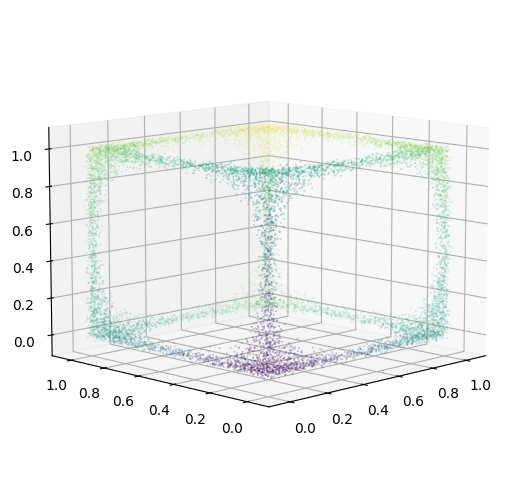
\includegraphics[width=0.9\linewidth]{python/plots/cube_points/data/matrix/cube_points_m24_n01}
    \end{subfigure}%

%    \vspace{0.5em}

    \begin{subfigure}[b]{0.25\textwidth}
        \centering
        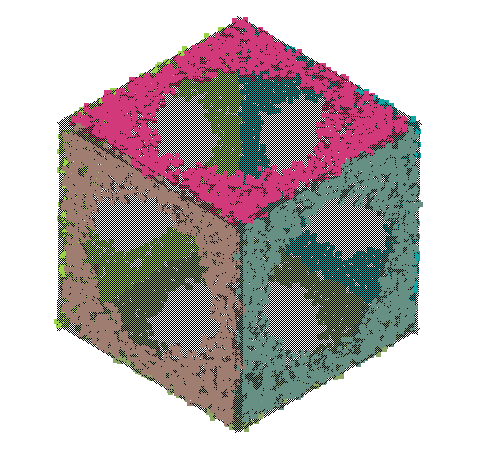
\includegraphics[width=0.9\linewidth]{python/plots/cube_points/data/matrix/cube_points_m6_n01_primitives}
        \caption{Missing level 6}
    \end{subfigure}%
    \begin{subfigure}[b]{0.25\textwidth}
        \centering
        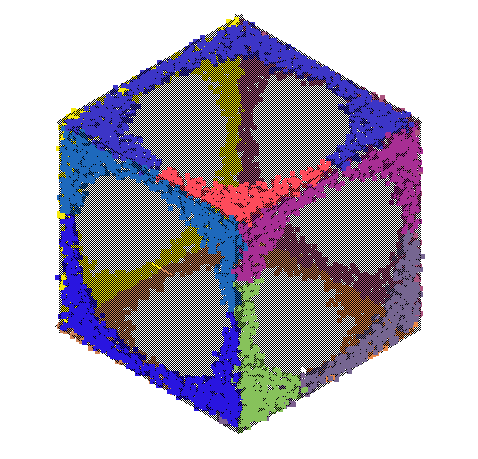
\includegraphics[width=0.9\linewidth]{python/plots/cube_points/data/matrix/cube_points_m12_n01_primitives}
        \caption{Missing level 12}
    \end{subfigure}%
    \begin{subfigure}[b]{0.25\textwidth}
        \centering
        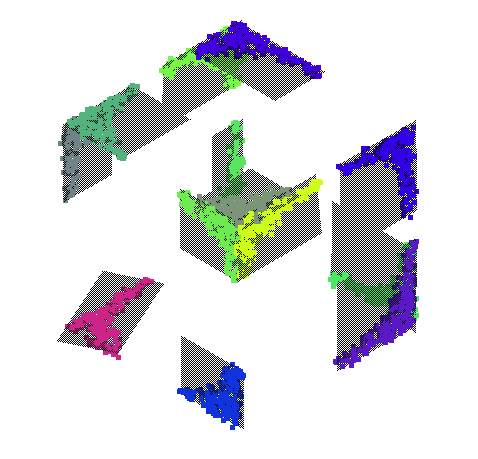
\includegraphics[width=0.9\linewidth]{python/plots/cube_points/data/matrix/cube_points_m24_n01_primitives}
        \caption{Missing level 24}
    \end{subfigure}%
    \caption{Unit cube with noise level = 0.01 and varying missing level}
    \label{fig:test-both}
\end{figure}

\subsection{Tests on real world data}\label{subsec:tests-on-real-world-data}
